% Options for packages loaded elsewhere
\PassOptionsToPackage{unicode}{hyperref}
\PassOptionsToPackage{hyphens}{url}
\documentclass[
  english,
  11pt,
  a4paper,
]{article}
\usepackage{xcolor}
\usepackage[margin=22mm,headheight=15pt]{geometry}
\usepackage{amsmath,amssymb}
\setcounter{secnumdepth}{-\maxdimen} % remove section numbering
\usepackage{iftex}
\ifPDFTeX
  \usepackage[T1]{fontenc}
  \usepackage[utf8]{inputenc}
  \usepackage{textcomp} % provide euro and other symbols
\else % if luatex or xetex
  \usepackage{unicode-math} % this also loads fontspec
  \defaultfontfeatures{Scale=MatchLowercase}
  \defaultfontfeatures[\rmfamily]{Ligatures=TeX,Scale=1}
\fi
\usepackage{lmodern}
\ifPDFTeX\else
  % xetex/luatex font selection
\fi
% Use upquote if available, for straight quotes in verbatim environments
\IfFileExists{upquote.sty}{\usepackage{upquote}}{}
\IfFileExists{microtype.sty}{% use microtype if available
  \usepackage[]{microtype}
  \UseMicrotypeSet[protrusion]{basicmath} % disable protrusion for tt fonts
}{}
\makeatletter
\@ifundefined{KOMAClassName}{% if non-KOMA class
  \IfFileExists{parskip.sty}{%
    \usepackage{parskip}
  }{% else
    \setlength{\parindent}{0pt}
    \setlength{\parskip}{6pt plus 2pt minus 1pt}}
}{% if KOMA class
  \KOMAoptions{parskip=half}}
\makeatother
\usepackage{longtable,booktabs,array}
\usepackage{caption}
\captionsetup[table]{skip=6pt}
\newcounter{none} % for unnumbered tables
\usepackage{calc} % for calculating minipage widths
% Correct order of tables after \paragraph or \subparagraph
\usepackage{etoolbox}
\makeatletter
\patchcmd\longtable{\par}{\if@noskipsec\mbox{}\fi\par}{}{}
\makeatother
\usepackage{graphicx}
\makeatletter
\newsavebox\pandoc@box
\newcommand*\pandocbounded[1]{% scales image to fit in text height/width
  \sbox\pandoc@box{#1}%
  \Gscale@div\@tempa{\textheight}{\dimexpr\ht\pandoc@box+\dp\pandoc@box\relax}%
  \Gscale@div\@tempb{\linewidth}{\wd\pandoc@box}%
  \ifdim\@tempb\p@<\@tempa\p@\let\@tempa\@tempb\fi% select the smaller of both
  \ifdim\@tempa\p@<\p@\scalebox{\@tempa}{\usebox\pandoc@box}%
  \else\usebox{\pandoc@box}%
  \fi%
}
% Set default figure placement to htbp
\def\fps@figure{htbp}
\makeatother
\ifLuaTeX
\usepackage[bidi=basic,shorthands=off]{babel}
\else
\usepackage[bidi=default,shorthands=off]{babel}
\fi
\ifLuaTeX
  \usepackage{selnolig} % disable illegal ligatures
\fi
\setlength{\emergencystretch}{3em} % prevent overfull lines
\providecommand{\tightlist}{%
  \setlength{\itemsep}{0pt}\setlength{\parskip}{0pt}}
% Scaling Law notes (English edition); style aligned with the Chinese edition.
\usepackage{fontspec}
\usepackage{enumitem}
\usepackage{fancyhdr}
\usepackage{fvextra}
\usepackage{etoolbox}
\usepackage{titlesec}

\setmainfont[
  Path=/usr/local/texlive/2026/texmf-dist/fonts/opentype/public/tex-gyre/,
  UprightFont=texgyrepagella-regular.otf,
  BoldFont=texgyrepagella-bold.otf,
  ItalicFont=texgyrepagella-italic.otf,
  BoldItalicFont=texgyrepagella-bolditalic.otf
]{texgyrepagella-regular.otf}
\setsansfont[
  Path=/usr/local/texlive/2026/texmf-dist/fonts/opentype/public/tex-gyre/,
  UprightFont=texgyreheros-regular.otf,
  BoldFont=texgyreheros-bold.otf,
  ItalicFont=texgyreheros-italic.otf,
  BoldItalicFont=texgyreheros-bolditalic.otf
]{texgyreheros-regular.otf}
\setmonofont[
  Path=/usr/local/texlive/2026/texmf-dist/fonts/opentype/google/roboto/,
  UprightFont=RobotoMono-Regular.otf,
  BoldFont=RobotoMono-Bold.otf,
  ItalicFont=RobotoMono-Italic.otf,
  BoldItalicFont=RobotoMono-BoldItalic.otf,
  Scale=0.82
]{RobotoMono-Regular.otf}

\definecolor{attentionblue}{HTML}{174A7E}
\definecolor{attentiongray}{HTML}{5D6773}
\definecolor{attentionlink}{HTML}{1769AA}
\definecolor{codebg}{HTML}{F4F6F8}

\AtBeginDocument{%
  \hypersetup{
    linkcolor=attentionblue,
    urlcolor=attentionlink,
    citecolor=attentionblue,
    pdftitle={Scaling Law: From Compute Allocation to Hyperparameter Prediction}
  }%
}

\titleformat{\section}
  {\LARGE\bfseries\sffamily\color{attentionblue}}{}{0pt}{}
\titleformat{\subsection}
  {\Large\bfseries\sffamily\color{attentionblue}}{}{0pt}{}
\titleformat{\subsubsection}
  {\large\bfseries\sffamily\color{attentiongray}}{}{0pt}{}
\titlespacing*{\section}{0pt}{1.8ex}{1.2ex}
\titlespacing*{\subsection}{0pt}{1.6ex}{0.9ex}
\titlespacing*{\subsubsection}{0pt}{1.4ex}{0.7ex}

\setlength{\parindent}{2em}
\setlength{\parskip}{0.35em}
\linespread{1.18}
\setlist{itemsep=0.25em,topsep=0.45em,leftmargin=2.4em}
\setcounter{tocdepth}{2}
\setcounter{secnumdepth}{0}

\pagestyle{fancy}
\fancyhf{}
\fancyhead[L]{\small\sffamily\color{attentiongray} Scaling Law}
\fancyhead[R]{\small\sffamily\color{attentiongray} Purshow's Notes}
\fancyfoot[C]{\small\sffamily\thepage}
\renewcommand{\headrulewidth}{0.3pt}


\usepackage{caption}
\captionsetup{font=small,labelfont=bf}
\clearcaptionsetup{table} % The overview has no caption.
\usepackage{float}
\floatplacement{figure}{H}

% A single opening page: article title above an automatically linked contents.
\makeatletter
\renewcommand*\l@subsection{\@dottedtocline{2}{0em}{0em}}
\renewcommand*\l@subsubsection{\@dottedtocline{3}{1.6em}{0em}}
\makeatother
\newcommand{\NotesCover}[1]{%
  \pagenumbering{roman}%
  \thispagestyle{empty}%
  \vspace*{0mm}%
  {\centering
    \sffamily\bfseries\color{attentionblue}%
    \fontsize{26pt}{36pt}\selectfont #1\par
  }%
  \vspace{4mm}%
  {\color{attentionblue}\noindent\rule{\linewidth}{0.6pt}\par}%
  \vspace{4mm}%
  \begingroup
    \setlength{\parindent}{0pt}%
    \setlength{\parskip}{0.6em}%
    \tableofcontents
  \endgroup
}
\newcommand{\NotesCoverEnd}{%
  \clearpage
  \pagenumbering{arabic}%
}

% Compact wrapping overview table, following Attention and MoE notes.
\newcommand{\OverviewTableStyle}{%
  \linespread{1}\fontsize{8.5pt}{10.5pt}\selectfont
  \setlength{\tabcolsep}{2.5pt}%
  \renewcommand{\arraystretch}{1.15}%
  \setlength{\extrarowheight}{6pt}%
  \setlength{\LTpre}{22pt}%
  \setlength{\LTpost}{0pt}%
  \setlength{\parskip}{0pt}%
}

% Keep the compact lookup flow together on one page.
\BeforeBeginEnvironment{verbatim}{\begin{samepage}}
\AfterEndEnvironment{verbatim}{\end{samepage}}

% Avoid isolated first or last lines at page boundaries.
\clubpenalty=10000
\widowpenalty=10000
\displaywidowpenalty=10000

% An unbreakable formula group keeps the introduction and display together.
\newenvironment{NotesFormula}{%
  \par\noindent\begin{minipage}{\linewidth}%
  \setlength{\parindent}{2em}%
  \setlength{\parskip}{0.35em}%
}{\end{minipage}\par}
\usepackage{bookmark}
\IfFileExists{xurl.sty}{\usepackage{xurl}}{} % add URL line breaks if available
\urlstyle{same}
% fallback for those not using the hyperref driver hyperxmp:
\makeatletter
\@ifundefined{xmpquote}{\newcommand{\xmpquote}[1]{#1}}{}
\makeatother
\hypersetup{
  pdflang={en},
  hidelinks,
  pdfcreator={LaTeX via pandoc}}

\author{}
\date{}

\begin{document}

\NotesCover{Scaling Law: From Compute Allocation to Hyperparameter Prediction}

\begingroup\OverviewTableStyle

{\def\LTcaptype{none} % do not increment counter
\begin{longtable}[]{@{}
  >{\centering\arraybackslash}p{(\linewidth - 6\tabcolsep) * \real{0.2000}}
  >{\centering\arraybackslash}p{(\linewidth - 6\tabcolsep) * \real{0.2400}}
  >{\centering\arraybackslash}p{(\linewidth - 6\tabcolsep) * \real{0.2700}}
  >{\centering\arraybackslash}p{(\linewidth - 6\tabcolsep) * \real{0.2900}}@{}}
\toprule\noalign{}
\begin{minipage}[b]{\linewidth}\centering
\textbf{Work}
\end{minipage} & \begin{minipage}[b]{\linewidth}\centering
\textbf{Date}
\end{minipage} & \begin{minipage}[b]{\linewidth}\centering
\textbf{Research Question}
\end{minipage} & \begin{minipage}[b]{\linewidth}\centering
\textbf{Core Method}
\end{minipage} \\
\midrule\noalign{}
\endhead
\bottomrule\noalign{}
\endlastfoot
\textbf{Rosenfeld et al.} & 2019.09 & How error varies jointly with
\(N,D\) & Joint power-law fit across architectures / optimizers \\
\textbf{Kaplan Law} & 2020.01 & How loss varies with \(N,D,C\) &
Power-law fit + Critical Batch Size correction \\
\textbf{Chinchilla Law} & 2022.03 & How to split a fixed \(C\) between
\(N,D\) & Envelope / IsoFLOP / Parametric Fit \\
\textbf{DeepSeek Law} & 2024.01 & Improved compute definition + how
hyperparameters vary with \(C\) & Non-Embedding FLOPs/token \(M\) +
IsoFLOP \\
\textbf{Microsoft Law} & 2024.09 & How the optimal LR varies with
\(N,D\) & LR Sweep + quadratic fit + power-law fit \\
\textbf{Step Law} & 2025.03 & Directly predict the optimal LR and BS &
Grid Search over 3,700+ models + OLS + Bootstrap \\
\textbf{Farseer} & 2025.06 & The interaction term between \(N,D\) &
Differential Piecewise Fitting \\
\textbf{MAI} & 2026.10 & How small-model experiments can transfer
reliably to large models & Scaling Ladder + fixed TPP + Source
Scaling \\
\end{longtable}
}

\endgroup

\NotesCoverEnd

\subsection{0. What Is a Scaling Law}\label{what-is-a-scaling-law}

We first present some useful concepts and common conclusions.

The concept of a Scaling Law is this: as model size, dataset size, and
compute resources increase, the training loss decreases in a predictable
way. This downward trend follows a power-law curve, which appears as a
straight line on a log-log plot. We can view Scaling Laws as a framework
describing the relationships among compute, loss, model size, and data.
Its core lies in how to allocate precious compute resources sensibly, so
as to strike the best balance among the various factors.

\subsubsection{Notation}\label{notation}

\(N\) is the number of model parameters; \(D\) is the number of training
tokens; \(C\) is the training compute (FLOPs); \(E\) is the irreducible
loss; \(L,\hat L(\cdot)\) are the test loss and its prediction function
(they may also refer to the training loss; the two are strongly
correlated); \(\epsilon\) is the generalization error.

\subsubsection{\texorpdfstring{Where Does the Common \(C\approx6ND\)
Come
From?}{Where Does the Common C\textbackslash approx6ND Come From?}}\label{where-does-the-common-capprox6nd-come-from}

Transformer computation is almost entirely matrix multiplication, and
passing one token through a weight matrix
\(W\in\mathbb R^{d_{\mathrm{in}}\times d_{\mathrm{out}}}\) costs
\(2d_{\mathrm{in}}d_{\mathrm{out}}\) FLOPs, i.e., \textbf{one
multiply-add per parameter = 2 FLOPs}:

\begin{itemize}
\tightlist
\item
  \textbf{Forward}: \(Y=XW\), \(2N\) per token;
\item
  \textbf{Backward}: two matrix multiplications of the same size,
  \(\partial\mathcal L/\partial X=GW^\top\) (passed to the previous
  layer) and \(\partial\mathcal L/\partial W=X^\top G\) (for updating
  the parameters), \(4N\) per token.
\end{itemize}

\[C\approx\underbrace{2ND}_{\text{forward}}+\underbrace{4ND}_{\text{backward}}=6ND.\]

Of course, this certainly omits some computation:

\begin{itemize}
\tightlist
\item
  \textbf{Attention's \(QK^\top\) and \(AV\)}: about \(4Sd\) forward per
  layer per token (\(S\) is the context length); its ratio to the weight
  term is about \(S/6d\), which is not negligible for long contexts.
  DeepSeek's \(M=72Ld^2+12LdS\) is the version that includes it.
\item
  \textbf{Embedding, Norm, Softmax, activations, residuals}: table
  lookups or \(O(d)\) element-wise operations, negligible compared with
  \(O(d^2)\).
\item
  \textbf{Optimizer updates}: once per step rather than once per token,
  negligible after amortization.
\end{itemize}

\subsubsection{Why Do We Like Power
Laws?}\label{why-do-we-like-power-laws}

\begin{NotesFormula}

Because after taking logarithms:

\[\log L=\log A-\alpha\log N\]

\end{NotesFormula}

it becomes a straight line.

This means we can fit a straight line on smaller models and then predict
the loss of larger models. \textbf{Power laws let Scaling Laws obtain
their parameters through simple regression fitting and thus extrapolate;
but whether the extrapolation is accurate depends on whether the power
law still holds at larger scales.}

\subsubsection{\texorpdfstring{Rosenfeld: A Joint Function of \(N\) and
\(D\)}{Rosenfeld: A Joint Function of N and D}}\label{rosenfeld-a-joint-function-of-n-and-d}

\begin{NotesFormula}

\href{https://arxiv.org/abs/1909.12673}{A Constructive Prediction of the
Generalization Error Across Scales} (Rosenfeld et al.~2020) studied this
question further. They attempted to treat the error as a joint function
of model size \(N\) and data size \(D\), while also examining the
effects of various architectures (ResNet, WRN, LSTM, Transformer) and
optimizers (Adam and various SGD variants) on the error. The empirical
results show that, with one of the variables fixed, the error decays as
a power law in the other:

\[\hat L(D,N)\approx\frac{A}{N^\alpha}+E_N,\qquad
\hat L(D,N)\approx\frac{B}{D^\beta}+E_D.\]

\end{NotesFormula}

\begin{NotesFormula}

These can be combined into a joint form:

\[\boxed{\hat L(N,D)=E+\frac{A}{N^\alpha}+\frac{B}{D^\beta}}\]

\end{NotesFormula}

where \(A>0,B>0,\alpha\ge0,\beta\ge0\) are scalar constants, and the
value of \(E\) is independent of both \(N\) and \(D\). It contains three
terms:

{\def\LTcaptype{none} % do not increment counter
\begin{longtable}[]{@{}cl@{}}
\toprule\noalign{}
\textbf{Term} & \textbf{Meaning} \\
\midrule\noalign{}
\endhead
\bottomrule\noalign{}
\endlastfoot
\(A/N^\alpha\) & Loss caused by insufficient model capacity \\
\(B/D^\beta\) & Loss caused by insufficient training data \\
\(E\) & Irreducible loss \\
\end{longtable}
}

\clearpage

\subsection{1. Kaplan et al.'s Scaling
Laws}\label{kaplan-et-al.s-scaling-laws}

\href{https://arxiv.org/abs/2001.08361}{Scaling Laws for Neural Language
Models} (Kaplan et al.~2020) popularized the concept of Scaling Laws in
the field of language models. They found that the relationships between
the cross-entropy test loss \(L\) and model size \(N\) (excluding the
embedding layers), dataset size \(D\), and training compute \(C\) all
follow power laws, holding across multiple orders of magnitude. These
findings are consistent with the earlier research in the previous
section, but Kaplan et al.~took Transformer language models as their
subject and ran larger-scale empirical experiments: model sizes ranged
from 768 to 1.5B non-embedding parameters (admittedly not large by
today's standards), and dataset sizes from 22M to 23B tokens. All
training in the paper used the same learning rate schedule: 3000 steps
of linear warmup, followed by cosine decay to zero.

{\def\LTcaptype{none} % do not increment counter
\begin{longtable}[]{@{}
  >{\centering\arraybackslash}p{(\linewidth - 4\tabcolsep) * \real{0.2185}}
  >{\centering\arraybackslash}p{(\linewidth - 4\tabcolsep) * \real{0.3613}}
  >{\centering\arraybackslash}p{(\linewidth - 4\tabcolsep) * \real{0.4202}}@{}}
\toprule\noalign{}
\begin{minipage}[b]{\linewidth}\centering
\textbf{Research Direction}
\end{minipage} & \begin{minipage}[b]{\linewidth}\centering
\textbf{Core Question}
\end{minipage} & \begin{minipage}[b]{\linewidth}\centering
\textbf{Main Conclusion}
\end{minipage} \\
\midrule\noalign{}
\endhead
\bottomrule\noalign{}
\endlastfoot
1. Model Scaling & How does parameter count \(N\) affect loss? &
\(L(N)\propto N^{-0.076}\) \\
2. Data Scaling & How does data size \(D\) affect loss? &
\(L(D)\propto D^{-0.095}\) \\
3. Compute Scaling & How does compute \(C\) affect loss? &
\(L(C_{\min})\propto C_{\min}^{-0.050}\) \\
4. Model Shape & How important are structural parameters such as Depth,
Width, and Heads? & With parameter count fixed, the effect is small
within a reasonable range \\
5. Overfitting & How do parameter count and data size jointly determine
loss? & The overfitting penalty depends mainly on \(N^{0.74}/D\) \\
6. Training Dynamics & How does loss decrease with training steps? & Fit
\(L(N,S_{\min})\) and study the Critical Batch Size \\
7. Compute-Optimal Scaling & With FLOPs fixed, how should parameter
count and token count be allocated? & \(N^*\propto C^{0.73}\),
\(D^*\propto C^{0.27}\) \\
\end{longtable}
}

\subsubsection{\texorpdfstring{The Joint Loss Function
\(L(N,D)\)}{The Joint Loss Function L(N,D)}}\label{the-joint-loss-function-lnd}

\begin{NotesFormula}

Studying \(N\) and \(D\) separately is not enough, because in actual
training both affect the loss simultaneously. In Section 4, Kaplan
proposes:

\[\boxed{L(N,D)=\left[\left(\frac{N_c}{N}\right)^{\alpha_N/\alpha_D}+\frac{D_c}{D}\right]^{\alpha_D}}\]

\end{NotesFormula}

It describes the lower bound on loss jointly determined by model
capacity and data size. There are two important conclusions here:

\begin{itemize}
\tightlist
\item
  When \(D\to\infty\), the loss is mainly determined by the parameter
  count \(N\).
\item
  When \(N\to\infty\), the loss is mainly determined by the data size
  \(D\).
\end{itemize}

\begin{NotesFormula}

The experiments also found that, to control the relative loss penalty
caused by overfitting, the data size roughly needs to satisfy:

\[D\propto N^{0.74}\]

\end{NotesFormula}

\subsubsection{Critical Batch Size}\label{critical-batch-size}

Batch size determines two costs of training: \textbf{the number of
training steps} (wall-clock time) and \textbf{the number of tokens
processed} (compute). Kaplan Law borrows the empirical relation of
McCandlish et al.~(2018) to characterize the tradeoff between the two,
and from it defines the Critical Batch Size.

\begin{NotesFormula}

\textbf{1. The empirical relation.} When training a model to the same
loss, there is an approximately fixed tradeoff between the number of
training steps and the number of tokens processed:

\[\boxed{\left(\frac{S}{S_{\min}}-1\right)\left(\frac{E}{E_{\min}}-1\right)=1}\]

\end{NotesFormula}

where \(S\) is the number of training steps needed to reach the target
loss, and \(S_{\min}\) is the theoretical minimum number of steps (when
the batch is infinitely large); \(E=BS\) is the cumulative number of
tokens processed, and \(E_{\min}\) is the theoretical minimum number of
tokens (when the batch is infinitely small).

\begin{NotesFormula}

\textbf{2. The tradeoff between small and large batches.} Substituting
\(E=BS\), the above can be rearranged as:

\[\boxed{S=S_{\min}+\frac{E_{\min}}{B}},\qquad
\boxed{E=E_{\min}+BS_{\min}}\]

\end{NotesFormula}

\begin{itemize}
\tightlist
\item
  Small batch: gradient noise is larger and more training steps are
  needed, but token utilization is efficient, with \(E\) close to
  \(E_{\min}\).
\item
  Large batch: gradient noise is smaller and fewer training steps are
  needed (\(S\) close to \(S_{\min}\)), but there are diminishing
  marginal returns: processing more tokens fails to reduce the number of
  steps significantly.
\end{itemize}

That is, \textbf{small batches are compute-efficient, while large
batches are step-efficient}, yet another tradeoff.

\begin{NotesFormula}

\textbf{3. Defining the Critical Batch Size.} To find the balance point
between the two efficiencies, set the two terms in
\(S=S_{\min}+E_{\min}/B\) equal, \(S_{\min}=E_{\min}/B\), which gives:

\[\boxed{B_{\mathrm{crit}}=\frac{E_{\min}}{S_{\min}}}\]

\end{NotesFormula}

At this point \(S=2S_{\min}\) and \(E=2E_{\min}\): both the steps and
the compute are only twice their respective theoretical optima. Hence:

\begin{itemize}
\tightlist
\item
  \(B\ll B_{\mathrm{crit}}\): increasing the batch significantly reduces
  the number of training steps while barely increasing compute.
\item
  \(B\gg B_{\mathrm{crit}}\): further increasing the batch yields little
  benefit, and compute waste is evident.
\end{itemize}

\begin{NotesFormula}

\textbf{4. The relationship between \(B_{\mathrm{crit}}\) and loss.}
Kaplan fits, through training experiments with different batch sizes:

\[\boxed{B_{\mathrm{crit}}(L)\propto L^{-4.76}}\]

\end{NotesFormula}

That is, \textbf{the lower the loss, the larger the Critical Batch
Size}: the further training progresses, the weaker the gradient signal
and the relatively larger the noise, so a larger batch is needed to
estimate the gradient effectively.

\subsubsection{How to Study the Compute-Optimal Scaling
Law?}\label{how-to-study-the-compute-optimal-scaling-law}

Goal: given a compute budget \(C\), how should model size, batch size,
and training steps be allocated to minimize loss? Research steps:

\begin{enumerate}
\def\labelenumi{\arabic{enumi}.}
\tightlist
\item
  \textbf{Correct for batch-size efficiency}: use \(B_{\mathrm{crit}}\)
  to convert the actual compute and training steps into their ideal
  minimum values.
\end{enumerate}

\[S_{\min}=\frac{S}{1+B_{\mathrm{crit}}/B},\qquad
C_{\min}=\frac{C}{1+B/B_{\mathrm{crit}}}\]

\begin{enumerate}
\def\labelenumi{\arabic{enumi}.}
\setcounter{enumi}{1}
\tightlist
\item
  \textbf{Fit the training curves}: study the loss corresponding to
  different model sizes and training steps.
\end{enumerate}

\[\boxed{L(N,S_{\min})=\left(\frac{N_c}{N}\right)^{\alpha_N}+\left(\frac{S_c}{S_{\min}}\right)^{\alpha_S}}\]

\begin{enumerate}
\def\labelenumi{\arabic{enumi}.}
\setcounter{enumi}{2}
\tightlist
\item
  \textbf{Fix the compute budget and find the optimal model size}:
\end{enumerate}

\[\min_{N,S_{\min}}L(N,S_{\min})\qquad
\text{s.t.}\quad C_{\min}=6NB_{\mathrm{crit}}(L)S_{\min}\]

\begin{NotesFormula}

By optimizing the joint function and fitting the optimal experimental
results under different budgets, we obtain:

\[\boxed{
\begin{aligned}
N_{\mathrm{opt}}&\propto C_{\min}^{0.73}\\
B_{\mathrm{crit}}&\propto C_{\min}^{0.24}\\
S_{\min}&\propto C_{\min}^{0.03}
\end{aligned}}\]

\end{NotesFormula}

Conclusion: Kaplan holds that when training compute increases, it should
be \textbf{used mainly to scale up the model size}, rather than to
significantly increase the number of training steps; optimal training
should stop before the model fully converges. (This is why we see models
around 2021 being almost freakishly large.)

The above are the classic original conclusions of Kaplan (2020); later,
Chinchilla (2022) corrected the growth ratio between the optimal model
size and the training tokens.

\clearpage

\subsection{2. Chinchilla}\label{chinchilla}

\href{https://arxiv.org/abs/2203.15556}{Training Compute-Optimal Large
Language Models} (Hoffmann et al.~2022) argues that Kaplan has two
problems:

\begin{enumerate}
\def\labelenumi{\arabic{enumi}.}
\tightlist
\item
  \textbf{The learning rate schedule problem.} Part of Kaplan's analysis
  relies on an LR schedule tied to a fixed training length, and uses
  intermediate losses during training to predict performance at shorter
  training durations. But when the target number of training tokens is
  small, if the learning rate still decays according to a longer
  training cycle, the learning rate has not yet decreased sufficiently
  at the intermediate checkpoints, so the loss may be too high, which
  affects the compute-optimal estimate.
\item
  \textbf{The model sizes are too small.} Kaplan's experiments include a
  large number of models with fewer than 100M parameters, whereas
  Chinchilla extends the scaling experiments to about 70M--16B
  parameters and observes that the optimal scaling curve may have some
  curvature. Therefore, extrapolating using only small models may
  introduce bias.
\end{enumerate}

\begin{NotesFormula}

Research question: given a fixed training compute budget \(C\), how many
model parameters \(N\) should be used, and how many tokens \(D\) should
be trained on, to obtain the lowest final pretraining loss?

\[\boxed{(N_{\mathrm{opt}},D_{\mathrm{opt}})=\mathop{\mathrm{argmin}}_{N,D}\,L(N,D)\quad\text{s.t.}\quad 6ND=C}\]

\end{NotesFormula}

Once \(C\) is fixed, there is necessarily a tradeoff between model size
and training tokens, \(D=C/(6N)\): the larger the model, the fewer
tokens are available for training. Chinchilla answers this question with
three approaches.

\subsubsection{1. Training Curve
Envelope}\label{training-curve-envelope}

\begin{enumerate}
\def\labelenumi{\arabic{enumi}.}
\tightlist
\item
  Train models with different parameter counts and record their loss
  curves as a function of FLOPs.
\item
  For each compute budget \(C\), find the model configuration with the
  lowest loss.
\item
  Fit how the optimal parameter count and tokens vary with compute.
\end{enumerate}

\begin{NotesFormula}

Conclusion:

\[N_{\mathrm{opt}}\propto C^{0.50},\qquad D_{\mathrm{opt}}\propto C^{0.50}\]

\end{NotesFormula}

\begin{center}

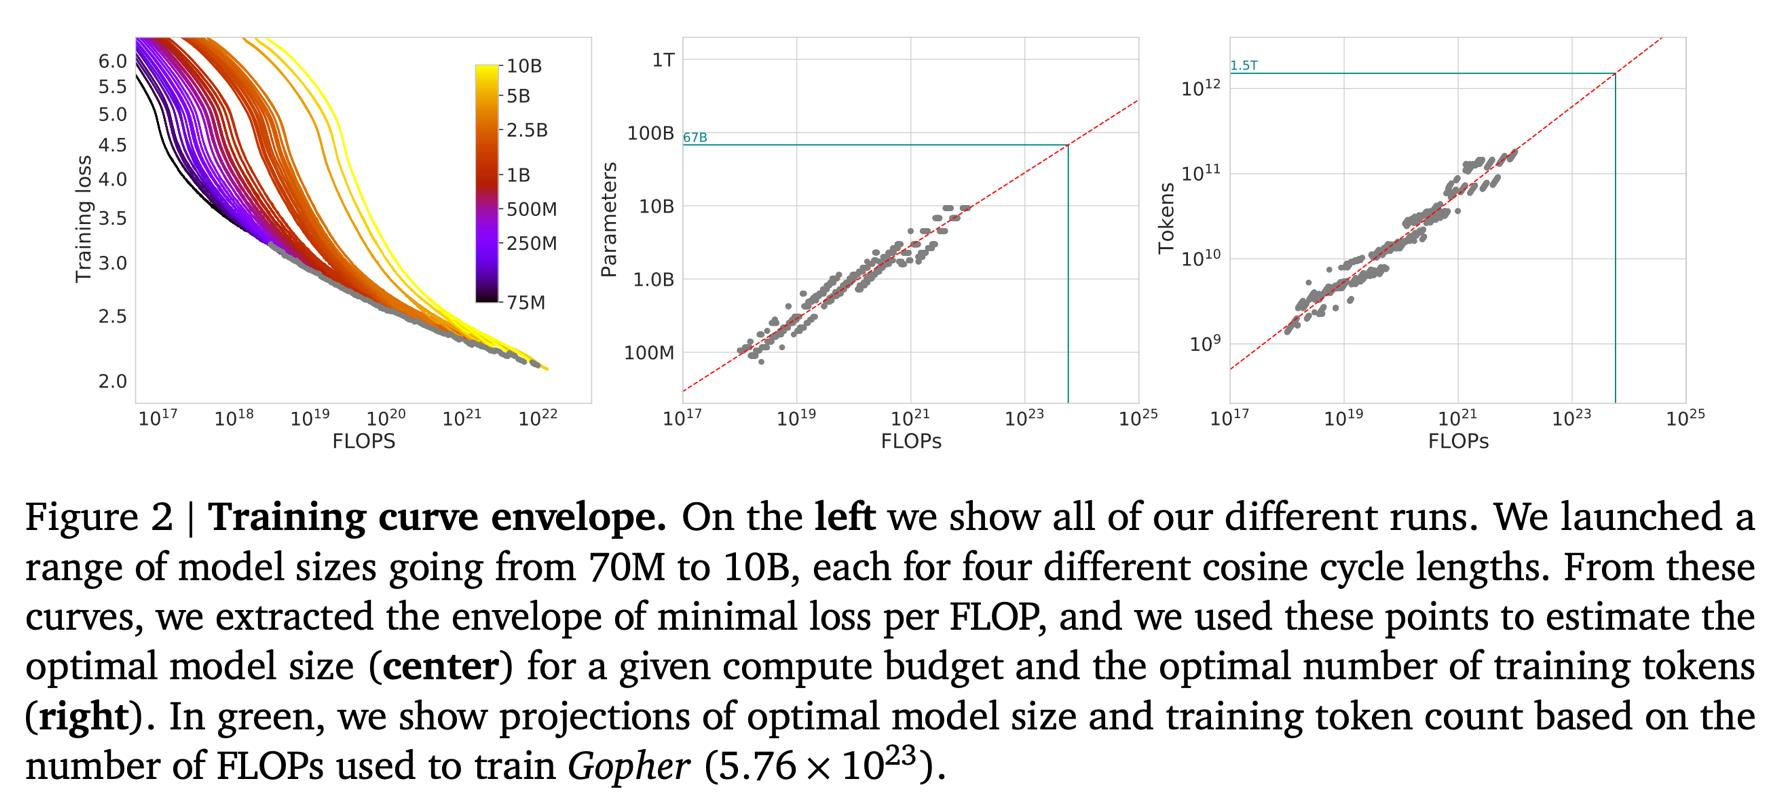
\includegraphics[width=0.72\linewidth,height=\textheight,keepaspectratio,alt={Chinchilla
Approach 1: Training Curve Envelope}]{assets/chinchilla-envelope.png}

\end{center}

\clearpage

\subsubsection{2. IsoFLOP (Fixed-Compute
Experiments)}\label{isoflop-fixed-compute-experiments}

\begin{enumerate}
\def\labelenumi{\arabic{enumi}.}
\tightlist
\item
  \textbf{Fix the compute budget \(C\)}: vary the model parameter count
  \(N\), while setting the training tokens \(D=C/(6N)\).
\item
  \textbf{Find the optimal configuration}: train all configurations and
  record the final loss, fit a quadratic curve to the experimental
  points; the minimum is \(N_{\mathrm{opt}}\), which gives
  \(D_{\mathrm{opt}}=C/(6N_{\mathrm{opt}})\).
\item
  \textbf{Fit the Scaling Law}: repeat the experiment for multiple
  values of \(C\) to obtain multiple sets of
  \((C,N_{\mathrm{opt}},D_{\mathrm{opt}})\), then perform a power-law
  fit.
\end{enumerate}

\begin{NotesFormula}

Conclusion:

\[\boxed{N_{\mathrm{opt}}\propto C^{0.49},\qquad D_{\mathrm{opt}}\propto C^{0.51}}\]

\end{NotesFormula}

Core: \textbf{two fits}. First use a quadratic curve to find the optimal
configuration at fixed FLOPs, then use a power law to fit the
relationship between the optimal configuration and FLOPs.

\begin{center}

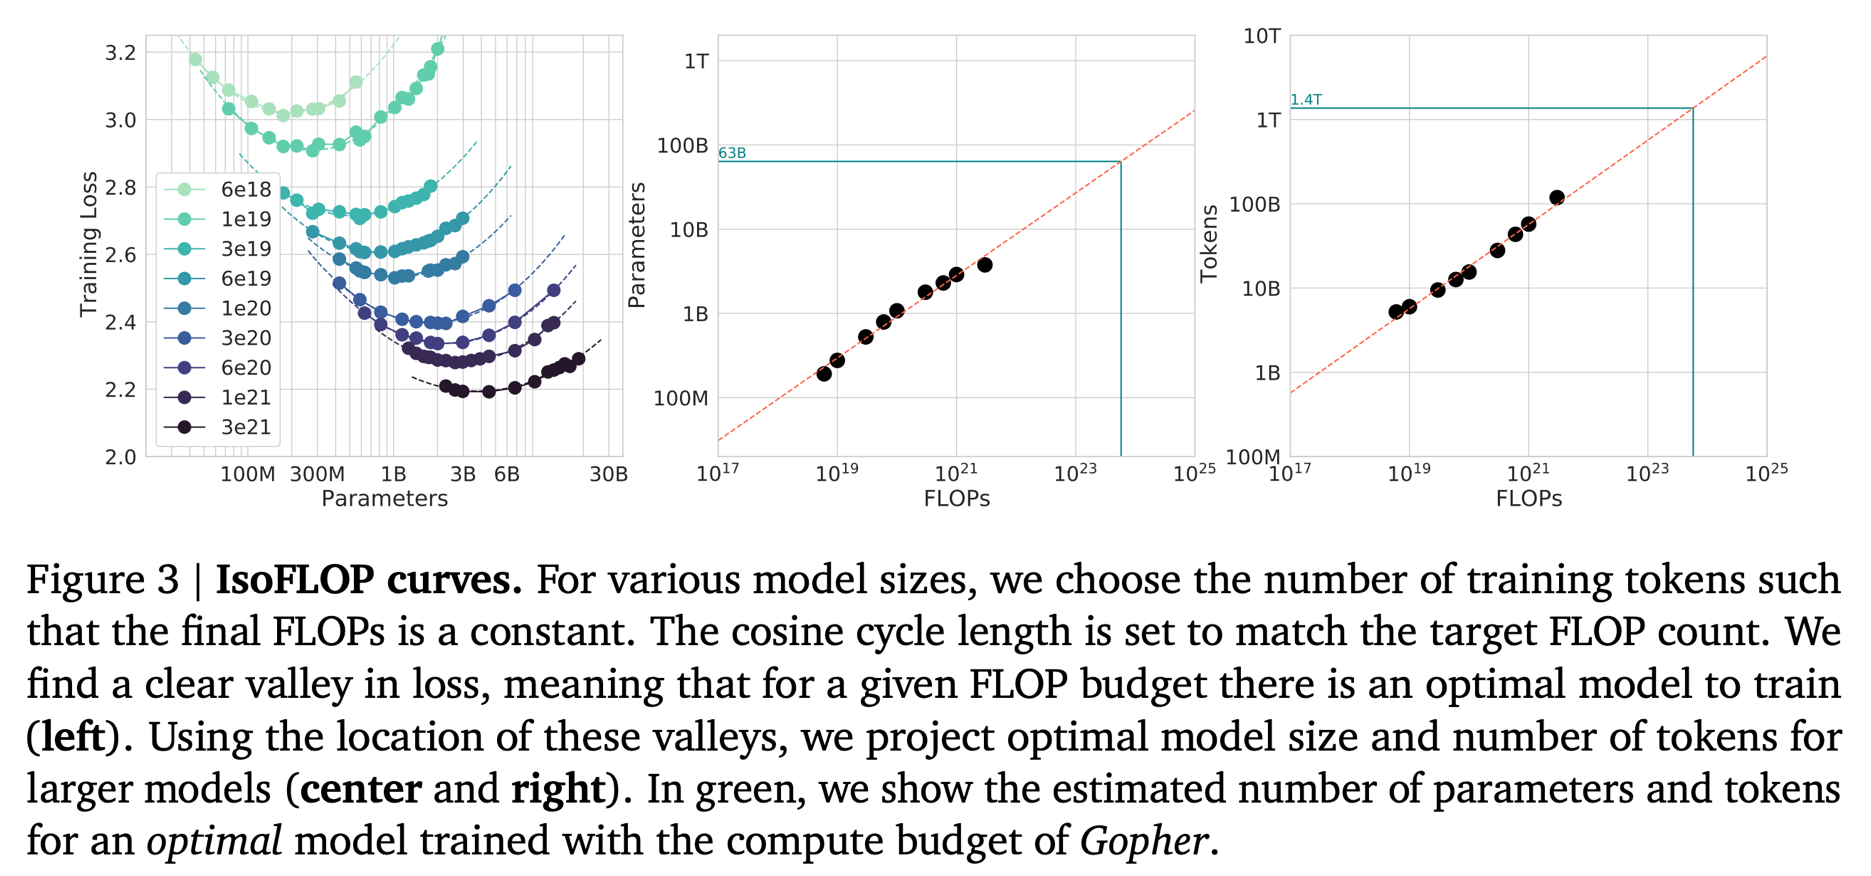
\includegraphics[width=0.72\linewidth,height=\textheight,keepaspectratio,alt={Chinchilla
Approach 2: IsoFLOP Curves}]{assets/chinchilla-isoflop.png}

\end{center}

\subsubsection{3. Parametric Loss
Function}\label{parametric-loss-function}

\begin{center}

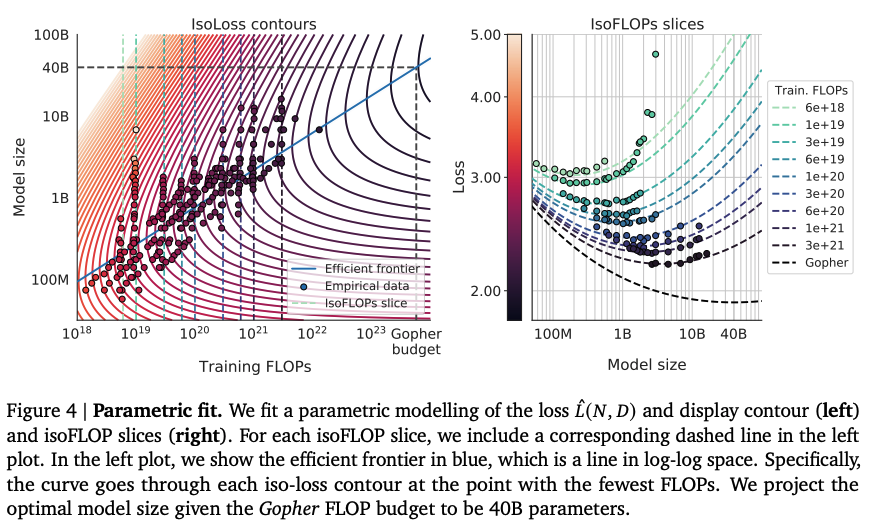
\includegraphics[width=0.8\linewidth,height=\textheight,keepaspectratio,alt={Chinchilla
Approach 3: Parametric Fit}]{assets/chinchilla-parametric.png}

\end{center}

\begin{enumerate}
\def\labelenumi{\arabic{enumi}.}
\tightlist
\item
  \textbf{Collect experimental data}: using the models trained in the
  first two approaches, collect the final training loss for different
  parameter counts \(N\) and training tokens \(D\), obtaining data
  points \((N_i,D_i,L_i)\).
\item
  \textbf{Fit the loss function}: assume the loss satisfies:
\end{enumerate}

\[L(N,D)=E+\frac{A}{N^\alpha}+\frac{B}{D^\beta}\]

\begin{NotesFormula}

where \(E\) is the irreducible loss, and the last two terms describe the
errors caused by finite model size and finite training data,
respectively. Use Huber Loss + L-BFGS to fit \(A,B,E,\alpha,\beta\):

\[\min_{\theta}\sum_i\operatorname{Huber}_{10^{-3}}\left(\log\hat L(N_i,D_i;\theta)-\log L_i\right)\]

\end{NotesFormula}

where \(\theta=(A,B,E,\alpha,\beta)\).

\begin{enumerate}
\def\labelenumi{\arabic{enumi}.}
\setcounter{enumi}{2}
\tightlist
\item
  \textbf{Solve for the optimal compute allocation}: fix the compute
  budget \(C=6ND\), and substitute \(D=C/(6N)\) into the fitted loss
  function:
\end{enumerate}

\[L(N)=E+\frac{A}{N^\alpha}+B\left(\frac{6N}{C}\right)^\beta\]

\begin{NotesFormula}

Differentiate with respect to \(N\) and set \(\frac{dL}{dN}=0\), which
gives:

\[N_{\mathrm{opt}}\propto C^{\frac{\beta}{\alpha+\beta}},\qquad
D_{\mathrm{opt}}\propto C^{\frac{\alpha}{\alpha+\beta}}\]

\end{NotesFormula}

\begin{NotesFormula}

Conclusion: the original paper's fit gives
\(\alpha\approx0.34,\beta\approx0.28\); computing with the unrounded
parameters:

\[\boxed{N_{\mathrm{opt}}\propto C^{0.46},\qquad D_{\mathrm{opt}}\propto C^{0.54}}\]

\end{NotesFormula}

\subsubsection{Core Differences Among the Three
Approaches}\label{core-differences-among-the-three-approaches}

\begin{NotesFormula}

Tokens per Parameter is defined as:

\[\boxed{R=\frac{D_{\mathrm{opt}}}{N_{\mathrm{opt}}}}\]

\end{NotesFormula}

The table below takes the compute budget of \emph{Gopher}
(\(5.76\times10^{23}\) FLOPs, corresponding to the 67B optimal model of
Approach 1) as an example, and compares the optimal model size, training
data size, and ratio recommended by the different approaches (values
taken from the Gopher projections in the three figures above).

{\def\LTcaptype{none} % do not increment counter
\begin{longtable}[]{@{}
  >{\centering\arraybackslash}p{(\linewidth - 10\tabcolsep) * \real{0.1350}}
  >{\centering\arraybackslash}p{(\linewidth - 10\tabcolsep) * \real{0.2025}}
  >{\centering\arraybackslash}p{(\linewidth - 10\tabcolsep) * \real{0.2025}}
  >{\centering\arraybackslash}p{(\linewidth - 10\tabcolsep) * \real{0.1840}}
  >{\centering\arraybackslash}p{(\linewidth - 10\tabcolsep) * \real{0.1840}}
  >{\centering\arraybackslash}p{(\linewidth - 10\tabcolsep) * \real{0.0920}}@{}}
\toprule\noalign{}
\begin{minipage}[b]{\linewidth}\centering
\textbf{Approach}
\end{minipage} & \begin{minipage}[b]{\linewidth}\centering
\(N_{\mathrm{opt}}\propto C^{a}\)
\end{minipage} & \begin{minipage}[b]{\linewidth}\centering
\(D_{\mathrm{opt}}\propto C^{b}\)
\end{minipage} & \begin{minipage}[b]{\linewidth}\centering
\textbf{\(N_{\mathrm{opt}}\)}
\end{minipage} & \begin{minipage}[b]{\linewidth}\centering
\textbf{\(D_{\mathrm{opt}}\)}
\end{minipage} & \begin{minipage}[b]{\linewidth}\centering
\textbf{\(R\)}
\end{minipage} \\
\midrule\noalign{}
\endhead
\bottomrule\noalign{}
\endlastfoot
Approach 1: Envelope & 0.50 & 0.50 & 67B & 1.5T & \(\approx22\) \\
Approach 2: IsoFLOP & 0.49 & 0.51 & 63B & 1.4T & \(\approx22\) \\
Approach 3: Parametric & 0.46 & 0.54 & 40B & \(\approx2.4\)T &
\(\approx60\) \\
Kaplan (2020) & 0.73 & 0.27 & - & - & - \\
\end{longtable}
}

Note: the \(D_{\mathrm{opt}}\) of Approach 3 is derived from
\(C/(6N_{\mathrm{opt}})\).

Interestingly, the later
\href{https://arxiv.org/abs/2404.10102}{Chinchilla Scaling: A
replication attempt} reconstructed the training data from the figures in
the Chinchilla paper and refit the Parametric Loss Function using Huber
Loss, finding that the original paper suffered from \textbf{premature
stopping of the optimizer}, \textbf{parameter precision problems
(rounding to two decimal places hurt it)}, and \textbf{overly narrow
confidence intervals for the scaling exponents}. The corrected scaling
exponents are \(0.513\) and \(0.487\), respectively, which are more
consistent with the first two approaches.

\subsubsection{Kaplan vs.~Chinchilla}\label{kaplan-vs.-chinchilla}

Why are their conclusions so different?

\begin{enumerate}
\def\labelenumi{\arabic{enumi}.}
\tightlist
\item
  \textbf{Kaplan's models are small}: a large number of experimental
  points fall in the sub-100M-parameter range, and the optimal scaling
  curve has curvature, so extrapolating the slope from the small-model
  range to large scales introduces bias.
\item
  \textbf{Embedding parameter count matters for small models.} Kaplan
  uses the non-embedding parameter count, while Chinchilla uses the
  total parameter count. For small models, embeddings make up a large
  share of the total parameters, so the two counting methods
  significantly change the fitted slope in the small-model range; the
  larger the model, the smaller this difference.
\end{enumerate}

{\def\LTcaptype{none} % do not increment counter
\begin{longtable}[]{@{}
  >{\centering\arraybackslash}p{(\linewidth - 4\tabcolsep) * \real{0.2105}}
  >{\centering\arraybackslash}p{(\linewidth - 4\tabcolsep) * \real{0.3684}}
  >{\centering\arraybackslash}p{(\linewidth - 4\tabcolsep) * \real{0.4211}}@{}}
\toprule\noalign{}
\begin{minipage}[b]{\linewidth}\centering
\end{minipage} & \begin{minipage}[b]{\linewidth}\centering
\textbf{Kaplan (2020)}
\end{minipage} & \begin{minipage}[b]{\linewidth}\centering
\textbf{Chinchilla (2022)}
\end{minipage} \\
\midrule\noalign{}
\endhead
\bottomrule\noalign{}
\endlastfoot
Model size & 768 -- 1.5B (non-embedding) & About 70M -- 16B \\
Parameter count & Non-embedding parameters & Total parameters \\
LR Schedule & Fixed cosine length, intermediate checkpoints taken &
Cosine cycle matched to the target training tokens \\
\(N_{\mathrm{opt}}\) & \(\propto C^{0.73}\) &
\(\propto C^{\approx0.5}\) \\
\(D_{\mathrm{opt}}\) & \(\propto C^{0.27}\) &
\(\propto C^{\approx0.5}\) \\
Practical advice & Spend compute primarily on scaling the model & Scale
model and data proportionally, about 20 Tokens/Param \\
\end{longtable}
}

\clearpage

\subsection{3. DeepSeek LLM}\label{deepseek-llm}

\href{https://arxiv.org/abs/2401.02954}{DeepSeek LLM: Scaling
Open-Source Language Models with Longtermism}

\subsubsection{Method: Following IsoFLOP, but with an Improved
Experimental
Setup}\label{method-following-isoflop-but-with-an-improved-experimental-setup}

Under a fixed compute budget \(C\), Chinchilla trains combinations of
different model sizes \(N\) and data sizes \(D\), finds the
configuration with the lowest loss, and then fits the compute-optimal
Scaling Law. DeepSeek follows this method but adds two improvements:

\begin{itemize}
\tightlist
\item
  \textbf{Non-Embedding FLOPs/token \(M\)}: use the non-embedding
  training compute per token instead of the parameter count \(N\) to
  measure model size:
\end{itemize}

\[M=72Ld^2+12LdS,\qquad C=MD\]

where \(L\) is the number of layers, \(d\) is the hidden size, and \(S\)
is the sequence length. Compared with directly using \(6N\), this
definition excludes vocabulary-related computation while accounting for
the computational cost of attention, making the compute estimates for
models of different sizes more accurate.

\begin{itemize}
\tightlist
\item
  \textbf{Hyperparameter Scaling}: first grid-search the batch size and
  learning rate on small models, treat configurations whose loss is
  within 0.25\% of the optimum as near-optimal, and then fit:
\end{itemize}

\[\boxed{
\begin{aligned}
B_{\mathrm{opt}}&=0.2920\,C^{0.3271}\\
\eta_{\mathrm{opt}}&=0.3118\,C^{-0.1250}
\end{aligned}}\]

That is, the larger the compute budget, the larger the optimal batch
size and the smaller the learning rate. They then extrapolate according
to the training compute budgets of 7B/67B to determine their BS and peak
LR.

\subsubsection{Conclusion: Broadly Supports Chinchilla, but Model Size
Grows Slightly
Faster}\label{conclusion-broadly-supports-chinchilla-but-model-size-grows-slightly-faster}

\begin{NotesFormula}

Both papers find that the optimal model size and data size grow
approximately as \(C^{0.5}\) with the compute budget:

\[\begin{aligned}
\text{Chinchilla:}\quad&N_{\mathrm{opt}}\propto C^{0.49},\quad D_{\mathrm{opt}}\propto C^{0.51}\\
\text{DeepSeek:}\quad&M_{\mathrm{opt}}\propto C^{0.5243},\quad D_{\mathrm{opt}}\propto C^{0.4757}
\end{aligned}\]

\end{NotesFormula}

\subsubsection{New Finding: Scaling Laws May Depend on Data
Quality}\label{new-finding-scaling-laws-may-depend-on-data-quality}

DeepSeek fit Scaling Laws separately on three datasets with different
quality and distributions, and found that as the data quality assessed
by the authors increased, the optimal growth exponent for model size
went \(0.450\to0.524\to0.578\), while the data exponent decreased
correspondingly. On this basis, the DeepSeek team argues that
\textbf{high-quality data may be better exploited by scaling up model
capacity}. However, this is an empirical correlation, and causality has
not been rigorously established.

\textbf{A brief summary}: Chinchilla established the compute-optimal
Scaling Law in which model and data grow in approximate balance;
building on this, DeepSeek improved the experimental methodology through
hyperparameter scaling and a more reasonable FLOPs definition, and
further found that the optimal scaling exponents may be affected by data
quality and distribution.

\clearpage

\subsection{4. Microsoft Law}\label{microsoft-law}

\href{https://arxiv.org/abs/2409.19913}{Scaling Optimal LR Across Token
Horizons} (Bjorck et al.~2024)

\textbf{Problem}: The existing method \(\mu\)P lets the optimal LR
transfer across model widths, but can it transfer across the
\textbf{Token Horizon} \(D\) (the total number of training tokens)? In
practice, one often sweeps the LR on short training runs and then uses
it directly for long training. This paper finds that doing so is wrong:
\textbf{the longer the training, the smaller the optimal LR, and it
decreases as a power law.}

\textbf{Method}: Run 250+ training runs on GPT-3-style models from 50M
to 2.7B, fitting in three steps:

\begin{enumerate}
\def\labelenumi{\arabic{enumi}.}
\tightlist
\item
  \textbf{Find the optimal LR}: fix \((N,D)\) and sweep the peak LR, fit
  \(L=a(\log\eta)^2+b\log\eta+c\), and take the minimum
  \(\eta^*=\exp(-b/2a)\).
\item
  \textbf{Fit the power law in \(D\)}: with \(N\) fixed, \(\log\eta^*\)
  is found to be linear in \(\log D\), i.e.,
  \(\eta^*(D)=A\,D^{-\beta}\).
\item
  \textbf{Combine \(N,D\)}: let \(\eta^*=C\,N^{-\alpha}D^{-\beta}\), fit
  using 760M--2.7B, and hold out 7B for validation (\(R^2=0.978\)).
\end{enumerate}

\begin{NotesFormula}

\textbf{Conclusion} (\(N,D\) in units of B; applicable to models
\(\geq 760\)M):

\[\boxed{\eta^*(N,D)\approx1.55\times10^{-3}\cdot N^{-0.23}\,D^{-0.32}}\]

\end{NotesFormula}

\begin{NotesFormula}

In practice, one only needs to find the optimal LR on a short training
run and then rescale proportionally:

\[\boxed{\eta^*(D_2)\approx\eta^*(D_1)\left(\frac{D_2}{D_1}\right)^{-0.32}}\]

\end{NotesFormula}

That is, for every 10× increase in training length, the optimal LR drops
to about 48\%.

\textbf{Findings}:

\begin{itemize}
\tightlist
\item
  \textbf{Extrapolatable}: using the results from 25B--100B to predict
  the optimal LR at 800B gives an error of about 10\%--15\%; directly
  reusing the LR from 100B gives an error of over 250\%.
\item
  \textbf{\(\mu\)P does not account for \(D\)}: \(\mu\)P only guarantees
  transfer across widths; even with \(\mu\)P, the optimal LR still
  decreases with \(D\).
\item
  \textbf{Batch size only shifts the curve}: a larger batch shifts the
  optimal LR upward overall, but the slope of its decrease with \(D\) is
  unchanged.
\item
  \textbf{Llama-1's LR was too large}: the extrapolated optimal LR for
  1T tokens is about \(1.1\times10^{-4}\), whereas \(3\times10^{-4}\)
  was actually used.
\end{itemize}

\clearpage

\subsection{5. Step Law}\label{step-law}

\href{https://arxiv.org/abs/2503.04715}{Predictable Scale: Part I, Step
Law -- Optimal Hyperparameter Scaling Law in Large Language Model
Pretraining}

A really excellent paper. Personally, I have always felt that Step's
research capability is underestimated by everyone.

Step Law directly predicts the optimal learning rate and batch size from
the model parameter count \(N\) and the number of training tokens \(D\).

\begin{center}

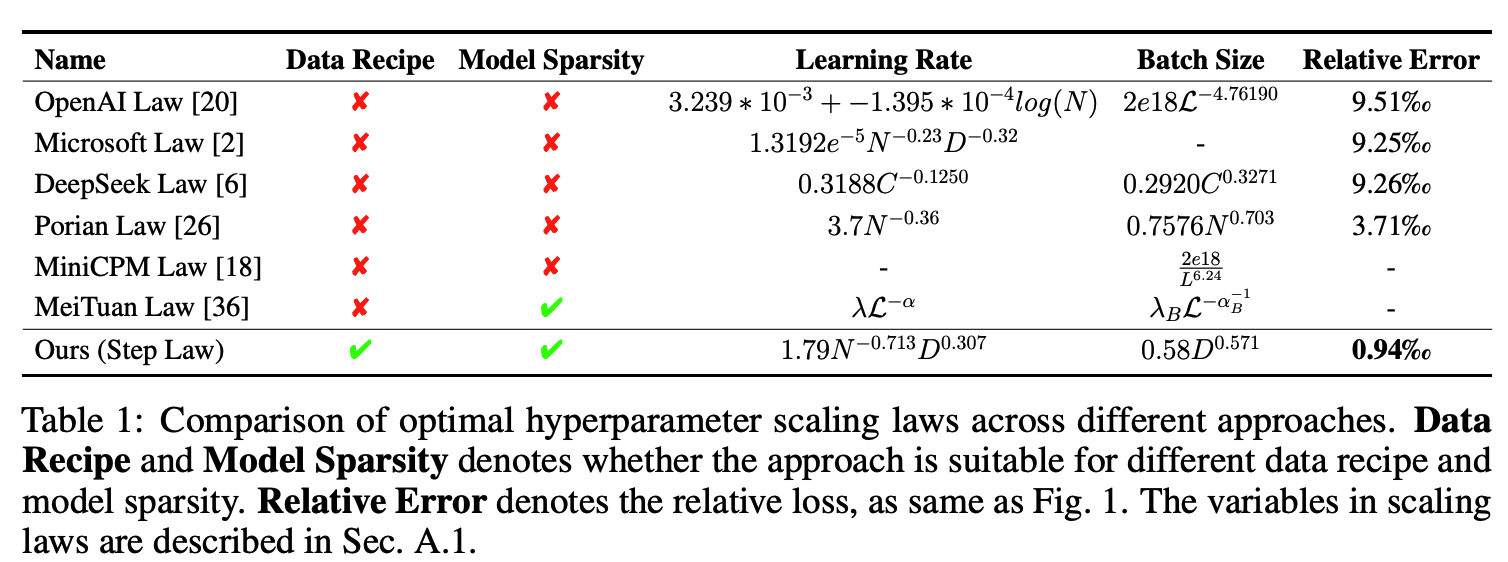
\includegraphics[width=0.95\linewidth,height=\textheight,keepaspectratio,alt={Comparison
of Step Law with existing hyperparameter Scaling
Laws}]{assets/steplaw-comparison.png}

\end{center}

\subsubsection{Problem Definition}\label{problem-definition}

\begin{NotesFormula}

The authors express the final training loss as:

\[\mathcal L(\mathbb A,\mathbb D,N,D,\eta,B)\]

\end{NotesFormula}

where:

\begin{itemize}
\tightlist
\item
  \(\mathbb A\): the model architecture.
\item
  \(\mathbb D\): the training data distribution.
\item
  \(N\): the non-embedding parameter count.
\item
  \(D\): the number of training tokens.
\item
  \(\eta\): the peak learning rate.
\item
  \(B\): the token-wise global batch size.
\end{itemize}

\begin{NotesFormula}

For a fixed model architecture, data distribution, and training scale,
the goal is:

\[(\eta^*,B^*)=\mathop{\arg\min}_{\eta,B}\,\mathcal L_{\mathbb A,\mathbb D,N,D}(\eta,B)\]

\end{NotesFormula}

\begin{NotesFormula}

Going further, they study whether there exist simple functions depending
only on \(N,D\):

\[\boxed{\eta^*=f(N,D),\qquad B^*=g(N,D)}\]

\end{NotesFormula}

\subsubsection{Experimental Scale}\label{experimental-scale}

\begin{itemize}
\tightlist
\item
  Over 3,700 LLMs trained from scratch.
\item
  About 100T tokens consumed in total.
\item
  Nearly 1 million NVIDIA H800 GPU-hours used.
\item
  Systematically varied the model parameter count, training data size,
  LR, BS, model shape, MoE sparsity, and data recipe.
\end{itemize}

The idea is: \textbf{first find the true optimal hyperparameters through
large-scale grid search, then study how these optima vary with \(N,D\),
and finally fit a Scaling Law with predictive power.}

\subsubsection{Grid Search Setup}\label{grid-search-setup}

The hyperparameter search mainly uses logarithmic spacing.

\begin{NotesFormula}

Learning rate:

\[\eta_i=2^{-10.5+0.5i},\qquad i=0,\ldots,7\]

\end{NotesFormula}

\begin{NotesFormula}

Batch size:

\[B_j=32768\cdot2^{j/2},\qquad j=0,\ldots,14\]

\end{NotesFormula}

Therefore:

\begin{itemize}
\tightlist
\item
  The learning rate has 8 candidate values.
\item
  The batch size has 15 candidate values.
\item
  The full \(8\times15\) grid search contains \textbf{120 hyperparameter
  combinations}.
\end{itemize}

For fixed \(N,D\), models with different LR and BS are each trained from
scratch, the final smoothed training loss is recorded, and the
hyperparameter combination with the lowest loss is identified.

In addition, Step \textbf{fixes the End LR at 1e-5}, whereas earlier
works such as DeepSeek usually set the End LR to a fixed fraction of the
peak LR (e.g., 10\%). But then, if the peak is high, it also drags the
end up, leaving the learning rate too high at the end of training? So
why not simply set the End LR to 0? Perhaps mainly to leave room for
later Mid/Post Train.

\subsubsection{Loss Landscape: An Approximately Convex
Bowl}\label{loss-landscape-an-approximately-convex-bowl}

\begin{center}

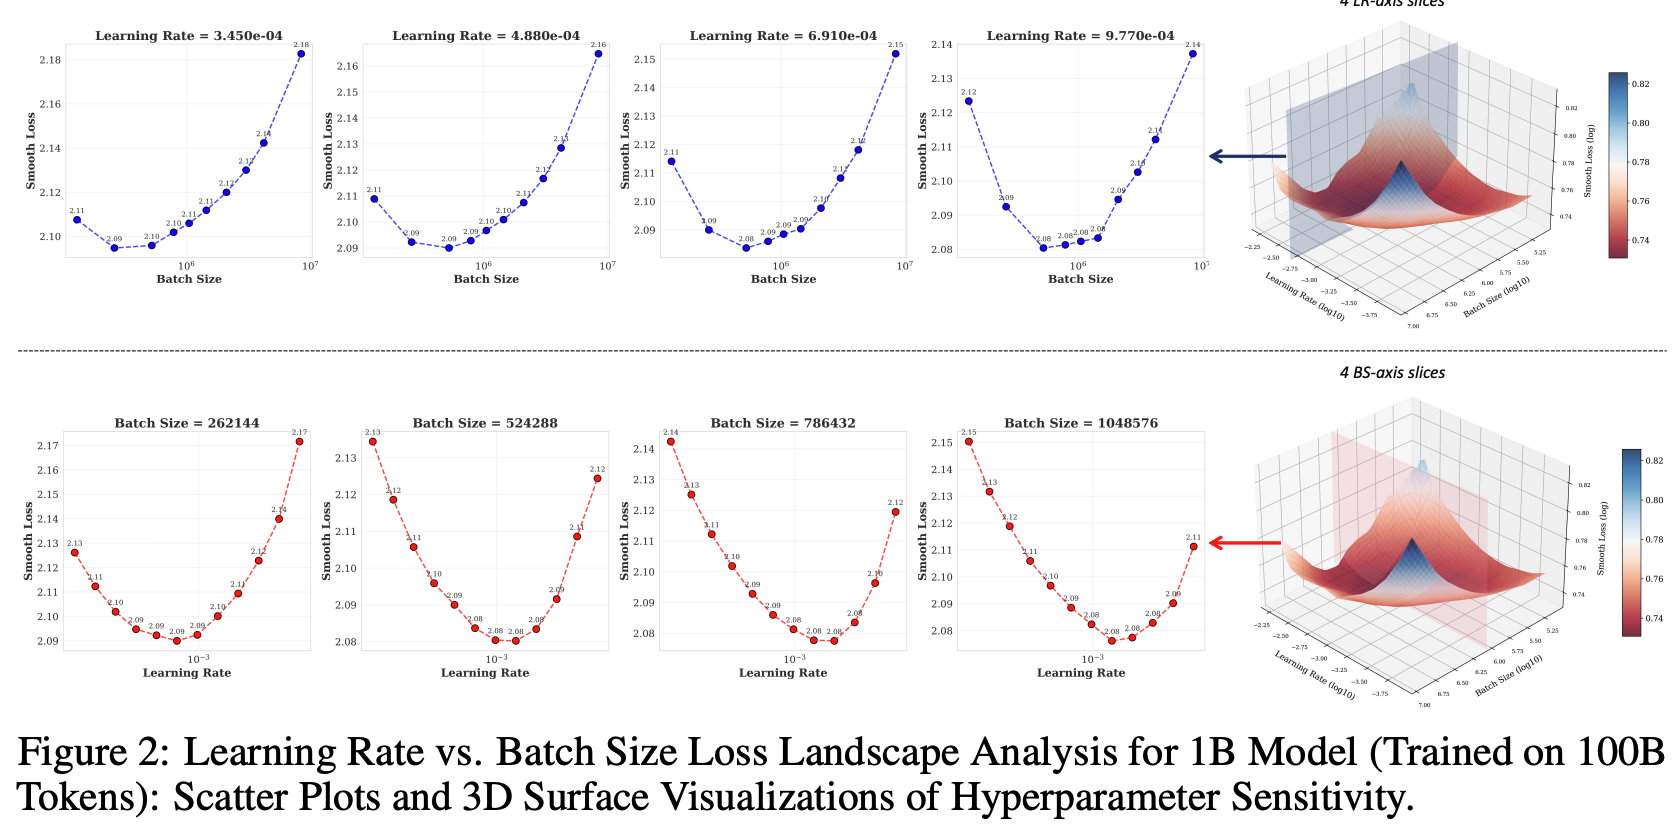
\includegraphics[width=0.95\linewidth,height=\textheight,keepaspectratio,alt={LR--BS
loss landscape of a 1B model (100B
tokens)}]{assets/steplaw-landscape.png}

\end{center}

\begin{itemize}
\tightlist
\item
  If the LR is too small, parameter updates are insufficient and
  convergence is slow.
\item
  If the LR is too large, training easily becomes unstable.
\item
  If the BS is too small, gradient noise is large.
\item
  If the BS is too large, the number of optimization steps under a given
  token budget decreases.
\end{itemize}

Therefore, in log LR--BS space, the loss usually exhibits an
approximately bowl-shaped structure: there is a low, approximately
convex loss landscape. This also puts us somewhat at ease: \textbf{the
prediction does not need to be all that precise to get close to the
optimal loss.}

\subsubsection{Fitting Step Law}\label{fitting-step-law}

\begin{center}

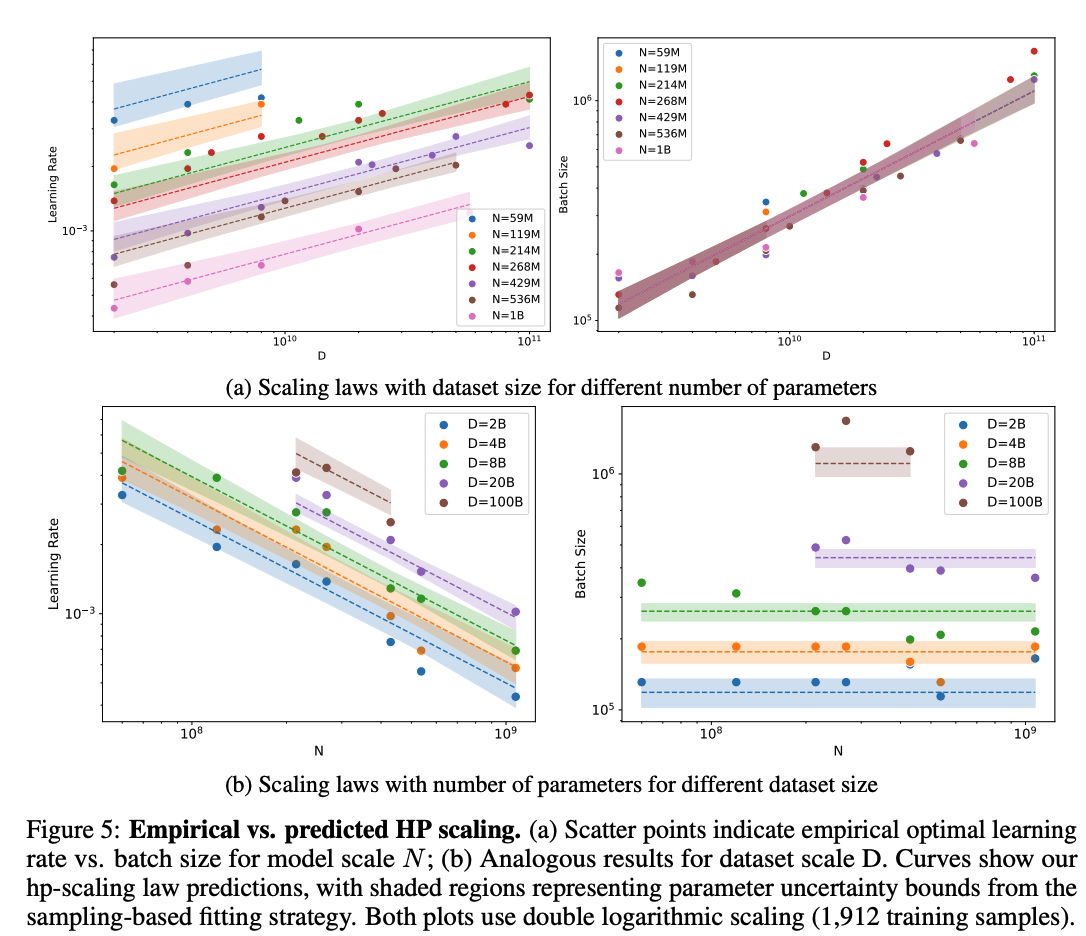
\includegraphics[width=0.88\linewidth,height=\textheight,keepaspectratio,alt={Empirically
optimal hyperparameters vs.~Step Law
predictions}]{assets/steplaw-fit.png}

\end{center}

Observe how the optimal hyperparameters trend with \(N,D\):

{\def\LTcaptype{none} % do not increment counter
\begin{longtable}[]{@{}
  >{\centering\arraybackslash}p{(\linewidth - 4\tabcolsep) * \real{0.2933}}
  >{\centering\arraybackslash}p{(\linewidth - 4\tabcolsep) * \real{0.3733}}
  >{\centering\arraybackslash}p{(\linewidth - 4\tabcolsep) * \real{0.3333}}@{}}
\toprule\noalign{}
\begin{minipage}[b]{\linewidth}\centering
\textbf{Controlled Variable}
\end{minipage} & \begin{minipage}[b]{\linewidth}\centering
\textbf{Optimal Learning Rate}
\end{minipage} & \begin{minipage}[b]{\linewidth}\centering
\textbf{Optimal Batch Size}
\end{minipage} \\
\midrule\noalign{}
\endhead
\bottomrule\noalign{}
\endlastfoot
Fix \(N\), increase \(D\) & Increases & Increases \\
Fix \(D\), increase \(N\) & Decreases & Roughly unchanged \\
\end{longtable}
}

\begin{NotesFormula}

Further observation in log-log coordinates shows the data points exhibit
an approximately linear relationship. Since:

\[\log y=a\log x+b\iff y=e^bx^a\]

\end{NotesFormula}

\begin{NotesFormula}

the authors therefore adopt the power-law forms:

\[\boxed{\eta(N,D)=cN^\alpha D^\beta},\qquad
\boxed{B(D)=dD^\gamma}\]

\end{NotesFormula}

where \(c,d,\alpha,\beta,\gamma\) are all parameters to be fitted.

\begin{NotesFormula}

\textbf{Log-Linear Regression + Bootstrap}: First, obtain the optimal
learning rate \(\eta^*\) and batch size \(B^*\) for different model
sizes \(N\) and training data sizes \(D\) through grid search; then take
logarithms to turn the power laws into linear relationships, and fit the
coefficients with OLS (ordinary least squares regression), i.e.,
minimize the squared error in log space between the predicted values and
the actual optimal hyperparameters. Finally, through 1000 rounds of
bootstrap resampling with replacement, repeat the fit and collect the
distribution of the coefficients to estimate the parameter uncertainty,
finally obtaining:

\[\boxed{\eta^*=1.79N^{-0.713}D^{0.307},\qquad B^*=0.58D^{0.571}}\]

\end{NotesFormula}

\clearpage

\subsection{6. Farseer}\label{farseer}

\textbf{Farseer: A Refined Scaling Law in Large Language Models}

Farseer argues that the traditional Chinchilla Scaling Law ignores the
interaction between the model parameter count \(N\) and the training
data size \(D\), and therefore proposes a new method for modeling the
loss surface \(L(N,D)\). Its key innovation is \textbf{making both the
coefficient and the exponent of data scaling depend on model size}, and
using Differential Piecewise Fitting to improve prediction and
extrapolation accuracy.

\begin{itemize}
\tightlist
\item
  Small models have limited capacity; even with more training data, they
  may be unable to effectively absorb more knowledge.
\item
  Large models have stronger representational power and can utilize data
  with different efficiency.
\item
  For models of different sizes, both the exponent and the coefficient
  of the data scaling curve may change simultaneously.
\end{itemize}

\begin{NotesFormula}

Starting from the general form:

\[\boxed{L(N,D)=E+U(N)+V(D)+H(N,D)}\]

\end{NotesFormula}

Compared with Chinchilla, an extra term \(H(N,D)\) is introduced,
representing \textbf{the interaction between parameter scale and data
scale that cannot be additively separated into two independent
functions}. Therefore, the core of the research shifts from fitting two
independent power laws to finding a more accurate, extrapolatable
two-dimensional loss surface.

However, \(H(N,D)\) cannot be observed independently and directly from
experiments, and fitting the four functions separately is also rather
difficult. The authors therefore design a fitting method that
\textbf{eliminates irrelevant terms through loss differences and
identifies the functional forms step by step}.

\subsubsection{Differencing: Eliminating the Terms We Don't Need to
Study}\label{differencing-eliminating-the-terms-we-dont-need-to-study}

\textbf{(1) Fix the model size \(N\), vary the data size \(D\)}

\begin{NotesFormula}

Define:

\[\Delta_DL(N,D)=L(N,D)-L(N,\lambda D)\]

\end{NotesFormula}

\begin{NotesFormula}

Expanding:

\[\begin{aligned}
\Delta_DL(N,D)={}&V(D)-V(\lambda D)\\
&+H(N,D)-H(N,\lambda D)
\end{aligned}\]

\end{NotesFormula}

We can see that \(E,\ U(N)\) are completely eliminated. Therefore,
\(\Delta_DL\) describes only the loss improvement brought by adding
training data.

\begin{NotesFormula}

If Chinchilla's independent additive form holds:

\[\Delta_DL(N,D)=BD^{-\beta}(1-\lambda^{-\beta})\]

\end{NotesFormula}

then this difference should be independent of \(N\). But experiments
find that \(\Delta_DL\) varies not only with \(D\) but also with \(N\).
This shows that \textbf{the data scaling law is model-size-dependent}.

\textbf{(2) Fix the data size \(D\), vary the model size \(N\)}

\begin{NotesFormula}

Similarly:

\[\Delta_NL(N,D)=L(N,D)-L(\lambda N,D)\]

\end{NotesFormula}

\begin{NotesFormula}

Expanding:

\[\begin{aligned}
\Delta_NL(N,D)={}&U(N)-U(\lambda N)\\
&+H(N,D)-H(\lambda N,D)
\end{aligned}\]

\end{NotesFormula}

This time \(E\) and \(V(D)\) are eliminated. If the effects of model
parameter count and data size were completely additively separable, this
difference should not depend on \(D\). But experiments likewise find a
clear dependence on data size.

\begin{center}

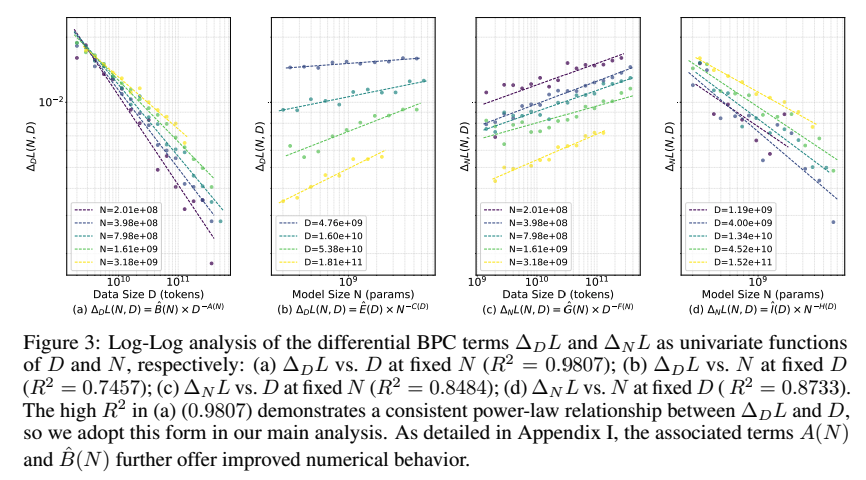
\includegraphics[width=0.95\linewidth,height=\textheight,keepaspectratio,alt={Log-log
analysis of the differential BPC term \textbackslash Delta\_DL versus
D}]{assets/farseer-differential.png}

\end{center}

\begin{NotesFormula}

The paper finds that with \(N\) fixed, \(\Delta_DL\) is approximately
linear in \(D\) in log-log coordinates (\(R^2=0.9807\)), and therefore
assumes:

\[\boxed{V(D)+H(N,D)\approx B(N)D^{-A(N)}}\]

\end{NotesFormula}

\subsubsection{Differential Piecewise
Fitting}\label{differential-piecewise-fitting}

\textbf{Stage 1: Differential + Log-Linear Regression}

\begin{NotesFormula}

Fix the model size \(N\), and take differences of the loss across
different data sizes to eliminate the model-size terms that are
independent of \(D\):

\[\begin{aligned}
R_N(D)&=L(N,D)-L(N,\lambda D)\\
&=B_N(1-\lambda^{-A_N})D^{-A_N}
\end{aligned}\]

\end{NotesFormula}

\begin{NotesFormula}

Taking logarithms:

\[\log R_N(D)=\log\hat B_N-A_N\log D\]

\end{NotesFormula}

Through linear regression, use the slope and intercept to solve for
\(A_N,B_N\) for each model size, where \(\lambda=\sqrt2\).

\textbf{Stage 2: Transformation Search + Iterative Fitting}

\begin{NotesFormula}

Perform a functional transformation search on the discrete \(A_N,B_N\)
obtained in Stage 1, finding that a stretched exponential fits best:

\[\boxed{
\begin{aligned}
A(N)&=\exp(a_1N^\alpha+b_1)\\
B(N)&=\exp(a_2N^\beta+b_2)
\end{aligned}}\]

\end{NotesFormula}

First determine the parameters via Grid Search + Linear Regression, then
alternately optimize \(\alpha,\beta\) to minimize the prediction error
of the overall loss differences.

\textbf{Stage 3: Residual Fitting}

\begin{NotesFormula}

The first two stages only fit the data-related term \(B(N)D^{-A(N)}\);
the model-size-related term still needs to be fitted. Subtract the
data-related term from the raw loss and average over different \(D\):

\[G(N)=\operatorname{Avg}_D\left[L(N,D)-B(N)D^{-A(N)}\right]\]

\end{NotesFormula}

\begin{NotesFormula}

Through another transformation search, we obtain:

\[\boxed{G(N)=E+U(N)\approx\exp(a_3N^\gamma+b_3)}\]

\end{NotesFormula}

\begin{NotesFormula}

\textbf{Final Scaling Law}

\[\boxed{L(N,D)=\exp(a_3N^\gamma+b_3)+\exp(a_2N^\beta+b_2)\,D^{-\exp(a_1N^\alpha+b_1)}}\]

\end{NotesFormula}

\begin{NotesFormula}

Substituting the values fitted in the paper:

\[\boxed{
\begin{aligned}
L(N,D)={}&\exp\!\left(-0.021N^{0.169}-0.091\right)\\
&+\exp\!\left(88.01N^{-0.1}-6.287\right)\cdot D^{-\exp\left(-0.124N^{0.123}+0.424\right)}
\end{aligned}}\]

\end{NotesFormula}

Here \(N\) is the actual number of parameters and \(D\) is the actual
number of tokens, rather than values substituted directly in units of B.

\textbf{Core advantage}: it decomposes a complex 9-parameter nonlinear
fit into multiple one-dimensional problems that are easier to solve,
reducing parameter coupling and sensitivity to initialization. In the
paper, compared with direct nonlinear regression, the relative fitting
error drops from 1.67\% to 0.18\%.

\clearpage

\subsection{7. MAI}\label{mai}

\href{https://microsoft.ai/pdf/mai-thinking-1.pdf}{MAI Thinking 1},
\href{https://microsoft.ai/news/frontier-pre-training-at-microsoft-ai/}{Frontier
Pre-training at Microsoft AI}

\subsubsection{1. Scaling Ladder}\label{scaling-ladder}

Build a series of models of different sizes that follow the same
architectural design rules and training recipe, and use small-model
experiments to guide large-model training.

\begin{itemize}
\tightlist
\item
  Each model's size is defined by its number of layers \(L\), and the
  other architectural parameters are determined by \(L\), e.g.,
  \(d_{\mathrm{model}}=\frac{256}{3}L\).
\item
  Progressively train models such as L18, L24, L30, L36, and L42.
\item
  Keep TPP constant, and control the number of data repetitions via
  Source Scaling.
\item
  Use the small-model experiments to fit a Scaling Law and predict the
  performance of the final MAI-Base-2.
\end{itemize}

\subsubsection{2. Tokens per Active Parameter
(TPP)}\label{tokens-per-active-parameter-tpp}

\begin{NotesFormula}

Defined as:

\[\boxed{TPP=\frac{D}{N_{\mathrm{active}}}}\]

\end{NotesFormula}

where:

\begin{itemize}
\tightlist
\item
  \(D\): the total number of tokens actually processed during training,
  including repeated data.
\item
  \(N_{\mathrm{active}}\): the number of parameters activated per token.
\end{itemize}

\begin{NotesFormula}

MAI-Base-2:

\[TPP=\frac{50\mathrm{T}}{80\mathrm{B}}=625\]

\end{NotesFormula}

TPP is kept fixed across the Scaling Ladder, i.e., by whatever factor
the model's active parameter count is scaled up, the training tokens are
scaled up by the same factor.

\textbf{Core purpose}: control the ratio of data size to active
parameter count across models of different sizes, making experiments at
different scales comparable.

\subsubsection{3. Source Scaling}\label{source-scaling}

\textbf{Problem}: Small models have shorter training horizons. If the
full dataset were used directly, small and large models would see
different numbers of data repetitions, which in turn produces different
overfitting pressures.

\textbf{Method}: Proportionally shrink the unique data of each dataset,
so that the number of repetitions of each data source remains consistent
across training scales. For example, in the full 50T training run, a
certain data source is repeated 8 times:

\begin{itemize}
\tightlist
\item
  Large model: uses the full unique dataset, repeated 8 times.
\item
  Small model: with a training horizon of 5T, uses only 1/10 of the
  original dataset, repeated 8 times.
\end{itemize}

\begin{NotesFormula}

Therefore:

\[D'_{\mathrm{unique}}=\frac{D'_{\mathrm{train}}}{D_{\mathrm{train}}}D_{\mathrm{unique}}\]

\end{NotesFormula}

\begin{NotesFormula}

At fixed TPP:

\[\boxed{\frac{D'_{\mathrm{unique}}}{N'_{\mathrm{active}}}=\frac{D_{\mathrm{unique}}}{N_{\mathrm{active}}}}\]

\end{NotesFormula}

\textbf{Core purpose}: simultaneously preserve both the number of data
repetitions and the ratio of unique data to active parameters,
preventing small models from favoring under-regularized architectures
and hyperparameters due to insufficient data repetition.

\subsubsection{4. How to Predict the Final
Loss?}\label{how-to-predict-the-final-loss}

\begin{enumerate}
\def\labelenumi{\arabic{enumi}.}
\tightlist
\item
  Build a Scaling Ladder and train models of different sizes, such as
  L18--L42.
\item
  Fix TPP and use Source Scaling to control the number of data
  repetitions.
\item
  Record each model's training FLOPs and held-out BPB.
\item
  Fit a Scaling Law between BPB and training FLOPs.
\item
  Extrapolate the fitted curve to the target model MAI-Base-2 to predict
  its final BPB.
\end{enumerate}

\begin{center}

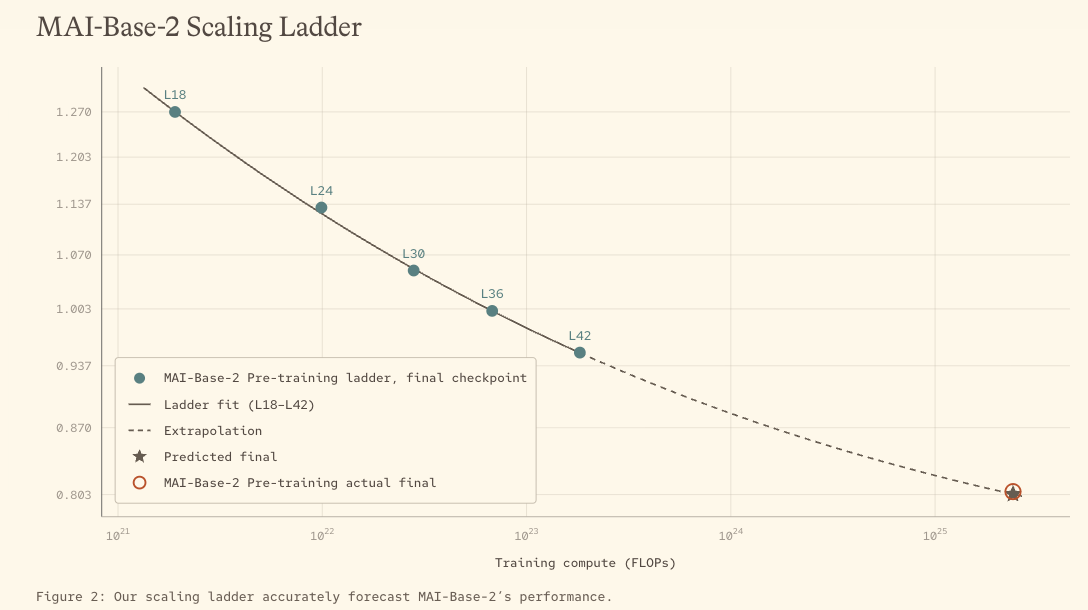
\includegraphics[width=0.88\linewidth,height=\textheight,keepaspectratio,alt={MAI-Base-2
Scaling Ladder}]{assets/mai-scaling-ladder.png}

\end{center}

\subsubsection{5. Efficiency Gain}\label{efficiency-gain}

\textbf{Problem}: Directly comparing the losses of two models conflates
the effects of model size, training compute, and training recipe.

\textbf{Method}: At the same evaluation loss, compare how much compute
each of the two models requires.

\begin{itemize}
\tightlist
\item
  \(EG_{\mathrm{FLOPs}}\): the efficiency multiple in FLOPs required to
  reach the same loss, measuring the computational efficiency of the
  algorithm and model design.
\item
  \(EG_{\mathrm{time}}\): the efficiency multiple in wall-clock time
  required to reach the same loss, measuring actual training-time
  efficiency, including the effects of the system implementation and
  hardware utilization.
\end{itemize}

\begin{NotesFormula}

Intuitively, the efficiency multiple can be understood as:

\[EG=\frac{C_{\mathrm{baseline}}}{C_{\mathrm{candidate}}}\]

\end{NotesFormula}

where \(C\) denotes the compute required to reach the same loss.
Microsoft mainly focuses on \(EG_{\mathrm{time}}\), because the actual
training cost depends on real-world running efficiency.

\begin{NotesFormula}

\textbf{Experimental results}: Fit a BPB--FLOPs Scaling Law separately
on each of four held-out evaluation sets, and back out the compute the
MAI recipe needs to reach the same BPB as DeepSeek-V4-Pro-Base.
MAI-Base-2 compared with DeepSeek-V4-Pro-Base:

\[\boxed{EG_{\mathrm{FLOPs}}=4.2\sim12.3\times}\]

\end{NotesFormula}

Of course, since a completely fair comparison is hard to achieve, this
number is bound to be biased toward MAI to some degree, and loss cannot
fully reflect model capability either.

\subsubsection{6. Hyperparameter Scaling
Laws}\label{hyperparameter-scaling-laws}

\textbf{Research goal}: Again, use small-model experiments to predict
the optimal LR, WD, and Dropout needed for large-scale pretraining,
reducing the cost of hyperparameter search for large models.

\textbf{(1) Joint LR and WD search}

\begin{NotesFormula}

The authors find that LR and WD are clearly coupled, and model
performance is especially sensitive to \(LR\times WD\). Therefore,
instead of a two-dimensional grid search directly over
\((\log LR,\log WD)\), they search jointly over:

\[\boxed{(\log LR,\ \log(LR\times WD))}\]

\end{NotesFormula}

\textbf{(2) Two-dimensional quadratic surface fit}

\begin{NotesFormula}

For the experimental results at different model sizes and TPPs, fit:

\[\mathcal L(x,y)=ax^2+by^2+cxy+dx+ey+f,\qquad
x=\log LR,\quad y=\log(LR\times WD)\]

\end{NotesFormula}

By solving for the analytical minimum of the surface, obtain the optimal
\((LR^*,\ LR^*\times WD^*)\).

\textbf{(3) Fitting the Hyperparameter Scaling Laws}

\begin{NotesFormula}

Using the optimal hyperparameters at different model sizes, TPPs, and
training steps, the fit gives:

\[\boxed{LR^*\times WD^*=\frac{17.04}{S}},\qquad
\boxed{\log LR^*=-1.51+0.175\log TPP-0.573\log S}\]

\end{NotesFormula}

where \(S\) is the total number of training steps. From this we get:

\begin{itemize}
\tightlist
\item
  \(LR^*\times WD^*\propto S^{-1}\): the more training steps, the
  smaller the product of LR and WD.
\item
  \(LR^*\propto S^{-0.573}\): the more training steps, the smaller the
  optimal LR.
\item
  \(LR^*\propto TPP^{0.175}\): with the number of training steps fixed,
  the larger the TPP, the larger the optimal LR.
\end{itemize}

\clearpage

\subsection{8. Comparing Optimal LR
Laws}\label{comparing-optimal-lr-laws}

The previous chapters all give Scaling Laws for the optimal LR, but at
first glance their conclusions contradict each other: for the same
increase in training data size \(D\), Microsoft Law says the optimal LR
decreases, while Step Law says it increases.

{\def\LTcaptype{none} % do not increment counter
\begin{longtable}[]{@{}
  >{\centering\arraybackslash}p{(\linewidth - 6\tabcolsep) * \real{0.1840}}
  >{\centering\arraybackslash}p{(\linewidth - 6\tabcolsep) * \real{0.3280}}
  >{\centering\arraybackslash}p{(\linewidth - 6\tabcolsep) * \real{0.2960}}
  >{\centering\arraybackslash}p{(\linewidth - 6\tabcolsep) * \real{0.1920}}@{}}
\toprule\noalign{}
\begin{minipage}[b]{\linewidth}\centering
\textbf{Work}
\end{minipage} & \begin{minipage}[b]{\linewidth}\centering
\textbf{Optimal LR Law}
\end{minipage} & \begin{minipage}[b]{\linewidth}\centering
\textbf{Batch Size}
\end{minipage} & \begin{minipage}[b]{\linewidth}\centering
\textbf{Experimental Conditions}
\end{minipage} \\
\midrule\noalign{}
\endhead
\bottomrule\noalign{}
\endlastfoot
\textbf{DeepSeek LLM} & \(\eta_{\mathrm{opt}}\propto C^{-0.125}\) &
\(B_{\mathrm{opt}}\propto C^{0.327}\) & Compute \(C\) as the independent
variable \\
\textbf{Microsoft Law} & \(\eta^*\propto N^{-0.23}D^{-0.32}\) & Fixed at
0.5M tokens & Only \(D\) varies; BS unchanged \\
\textbf{Step Law} & \(\eta^*\propto N^{-0.713}D^{+0.307}\) &
\(B^*\propto D^{0.571}\) & LR and BS both set to their optima \\
\textbf{MAI} & \(LR^*\propto TPP^{0.175}\,S^{-0.573}\) & --- & Separates
TPP from the step count \(S\) \\
\end{longtable}
}

\textbf{The contradiction comes from whether the batch size changes with
\(D\).} The number of training steps is \(S=D/B\), and the optimal LR is
mainly determined by the number of steps:

\begin{itemize}
\tightlist
\item
  \textbf{Microsoft Law}: \(B\) is fixed, \(S\propto D\), so the number
  of steps grows linearly with data size and the optimal LR decreases.
\item
  \textbf{Step Law}: \(B^*\propto D^{0.571}\), so the number of steps
  grows only as \(S\propto D^{0.429}\); meanwhile, a larger batch means
  smaller gradient noise, which in turn permits a larger LR. Combining
  the two, the optimal LR actually increases.
\item
  \textbf{DeepSeek}: by the same logic, as compute increases the optimal
  BS increases with it, and the optimal LR decreases only slowly
  (exponent of only \(-0.125\)).
\end{itemize}

\textbf{MAI's form separates the two effects}: the more steps, the
smaller the optimal LR (\(S^{-0.573}\)); with the number of steps fixed,
the more tokens each parameter sees (equivalent to a larger batch), the
larger the optimal LR (\(TPP^{0.175}\)). Roughly plugging in Microsoft
Law's setup (fixed \(N\) and \(B\), so \(TPP\propto D\) and
\(S\propto D\)) gives \(LR^*\propto D^{0.175-0.573}=D^{-0.40}\), of a
similar magnitude to Microsoft Law's \(D^{-0.32}\).

\textbf{References}

{[}1{]} Rosenfeld et al.: \href{https://arxiv.org/abs/1909.12673}{A
Constructive Prediction of the Generalization Error Across Scales}

{[}2{]} Kaplan et al.: \href{https://arxiv.org/abs/2001.08361}{Scaling
Laws for Neural Language Models}

{[}3{]} Hoffmann et al.:
\href{https://arxiv.org/abs/2203.15556}{Training Compute-Optimal Large
Language Models}

{[}4{]} DeepSeek-AI: \href{https://arxiv.org/abs/2401.02954}{DeepSeek
LLM: Scaling Open-Source Language Models with Longtermism}

{[}5{]} Besiroglu et al.:
\href{https://arxiv.org/abs/2404.10102}{Chinchilla Scaling: A
replication attempt}

{[}6{]} Bjorck et al.: \href{https://arxiv.org/abs/2409.19913}{Scaling
Optimal LR Across Token Horizons}

{[}7{]} StepFun: \href{https://arxiv.org/abs/2503.04715}{Predictable
Scale: Part I, Step Law -- Optimal Hyperparameter Scaling Law in Large
Language Model Pretraining}

{[}8{]} Li et al.: \href{https://arxiv.org/abs/2506.10972}{Predictable
Scale: Part II, Farseer: A Refined Scaling Law in Large Language Models}

{[}9{]} Lilian Weng:
\href{https://lilianweng.github.io/posts/2026-06-24-scaling-laws/}{Scaling
Laws}

{[}10{]} Su Jianlin:
\href{https://kexue.fm/archives/11833}{Deconstructing Scaling Law: A
Trio of Optimization, Architecture, and Data} (in Chinese)

{[}11{]} Stanford CS336: Lecture 09, Lecture 11 (Scaling Laws)

{[}12{]} Microsoft AI:
\href{https://microsoft.ai/pdf/mai-thinking-1.pdf}{MAI Thinking 1}

{[}13{]} Microsoft AI:
\href{https://microsoft.ai/news/frontier-pre-training-at-microsoft-ai/}{Frontier
Pre-training at Microsoft AI}

\end{document}
